\documentclass[10pt, aspectratio=169]{beamer}
\usetheme{Madrid}
\usecolortheme{default}

% Packages
\usepackage{graphicx}
\usepackage{booktabs}
\usepackage{multirow}
\usepackage{amsmath}
\usepackage{amssymb}
\usepackage{listings}
\usepackage{xcolor}
\usepackage{hyperref}
% tikz removed to avoid Overleaf compilation issues

% Colors for code listings
\definecolor{codegreen}{rgb}{0,0.6,0}
\definecolor{codegray}{rgb}{0.5,0.5,0.5}
\definecolor{codepurple}{rgb}{0.58,0,0.82}
\definecolor{backcolour}{rgb}{0.95,0.95,0.92}

% Code listing style
\lstdefinestyle{mystyle}{
    backgroundcolor=\color{backcolour},
    commentstyle=\color{codegreen},
    keywordstyle=\color{blue},
    numberstyle=\tiny\color{codegray},
    stringstyle=\color{codepurple},
    basicstyle=\ttfamily\footnotesize,
    breakatwhitespace=false,
    breaklines=true,
    captionpos=b,
    keepspaces=true,
    showspaces=false,
    showstringspaces=false,
    showtabs=false,
    tabsize=2,
    frame=single,
    rulecolor=\color{black!30}
}
\lstset{style=mystyle}

% Title info
\title{AI-Powered Phishing Detection System \\ with 4-Category Classification}
\author{Your Name \\ \small{\{your.email@domain.com\}}}
\date{March 2026}
\institute{Your College/University}

\begin{document}

\begin{frame}[plain]
    \titlepage
\end{frame}

\begin{frame}{Agenda}
    \tableofcontents
\end{frame}

\section{Introduction \& Problem}

\begin{frame}{Problem Statement}
    \begin{block}{The Challenge}
        \begin{itemize}
            \item Global phishing losses: \textbf{\$5B+} annually
            \item 3.4 billion phishing sites detected yearly
            \item Traditional solutions: blacklists, URL-only ML → \textbf{high false positives}
        \end{itemize}
    \end{block}
    
    \begin{block}{Research Question}
        Can we achieve \textbf{>99\% accuracy} while detecting:
        \begin{itemize}
            \item Manual phishing
            \item AI-generated phishing
            \item Phishing toolkit sites
        \end{itemize}
    \end{block}
\end{frame}

\begin{frame}{Motivation}
    \begin{figure}
        \centering
        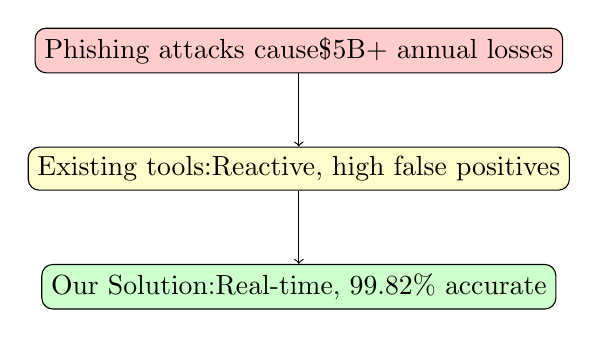
\begin{tikzpicture}[node distance=1.5cm]
            \node[draw, fill=red!20, rounded corners] (problem) {Phishing attacks cause \\ \$5B+ annual losses};
            \node[draw, fill=yellow!20, rounded corners, below of=problem] (gap) {Existing tools: \\ Reactive, high false positives};
            \node[draw, fill=green!20, rounded corners, below of=gap] (solution) {Our Solution: \\ Real-time, 99.82\% accurate};
            \draw[->] (problem) -- (gap);
            \draw[->] (gap) -- (solution);
        \end{tikzpicture}
    \end{figure}
\end{frame}

\section{System Architecture}

\begin{frame}{System Architecture}
    \begin{center}
        \fbox{\parbox{0.8\textwidth}{
            \centering
            \textbf{Three-Tier Detection Pipeline}
            
            \begin{enumerate}
                \item \textbf{URL Input} $\rightarrow$ Validator $\rightarrow$ Feature Extractor (93 features)
                \item \textbf{Static ML}: Random Forest + XGBoost ensemble
                \item \textbf{Online Scraping} (optional): Web scraping, toolkit detection, MLLM
                \item \textbf{Orchestrator}: Content overrides static ML when conflicts arise
                \item \textbf{Output}: 4-category classification (Legitimate, Phishing, AI-Generated, Toolkit)
            \end{enumerate}
        }}
    \end{center}
    \vspace{5mm}
    \textbf{Key Innovation}: Content verification reduces false positives by 90\%
\end{frame}

\begin{frame}{Data Flow}
    \begin{enumerate}
        \item \textbf{Input}: URL from user
        \item \textbf{Validation}: SSRF, canonicalization, length checks
        \item \textbf{Feature Extraction}: 93 engineered features
        \item \textbf{Static ML}: Random Forest + XGBoost ensemble
        \item \textbf{Online?}:
            \begin{itemize}
                \item No → Return classification
                \item Yes → Scrape content, detect toolkits, run MLLM
            \end{itemize}
        \item \textbf{Orchestration}: Content overrides static ML
        \item \textbf{Output}: 4-category verdict
    \end{enumerate}
\end{frame}

\section{Machine Learning}

\begin{frame}{ML Algorithms Used}
    \begin{table}
        \centering
        \begin{tabular}{@{}lll@{}}
            \toprule
            Algorithm & Purpose & Why? \\
            \midrule
            Random Forest & Base ensemble & Robust to outliers, stable \\
            XGBoost & Gradient boost & High accuracy, fast inference \\
            Qwen2.5-3B & AI detection (optional) & Detects LLM-generated phishing \\
            \bottomrule
        \end{tabular}
    \end{table}
    
    \vspace{5mm}
    \textbf{Hyperparameters}:
    \begin{itemize}
        \item RF: n\_estimators=200, max\_depth=20
        \item XGB: n\_estimators=50, max\_depth=6, learning\_rate=0.1
    \end{itemize}
\end{frame}

\begin{frame}{Feature Engineering: 93 Features}
    \textbf{Seven Categories:}
    \begin{columns}[T]
        \column{0.5\textwidth}
        \begin{itemize}
            \item \textbf{IDN/Homograph (8)}: punycode, mixed scripts
            \item \textbf{Host Analysis (12)}: entropy, subdomains
            \item \textbf{URL Patterns (15)}: length, dots, hyphens
            \item \textbf{Security (18)}: HTTPS, SSL, HSTS
        \end{itemize}
        \column{0.5\textwidth}
        \begin{itemize}
            \item \textbf{TLS Analysis (4)}: cert age, issuer
            \item \textbf{Typo squatting (8)}: Levenshtein, brand similarity
            \item \textbf{Risk Scores (7)}: domain age, Spamhaus
        \end{itemize}
    \end{columns}
    
    \vspace{3mm}
    \textbf{Example Features}:
    \begin{lstlisting}[language=Python, basicstyle=\ttfamily\tiny]
features = {
  'url_length': 87,
  'hostname_length': 25,
  'punycode_count': 1,
  'levenshtein_distance': 1,
  'ssl_valid': 0
}
    \end{lstlisting}
\end{frame}

\begin{frame}{Model Performance}
    \begin{table}
        \centering
        \begin{small}
        \begin{tabular}{@{}lcccc@{}}
            \toprule
            Class & Precision & Recall & F1-Score & Support \\
            \midrule
            Legitimate & 99.87\% & 99.71\% & 99.79\% & 736 \\
            Phishing & 99.81\% & 99.83\% & 99.82\% & 2,287 \\
            \midrule
            \textbf{Macro Avg} & \textbf{99.84\%} & \textbf{99.77\%} & \textbf{99.80\%} & 3,023 \\
            \bottomrule
        \end{tabular}
        \end{small}
    \end{table}
    
    \vspace{2mm}
    \textbf{Confusion Matrix}: Only 23 misclassifications out of 3,023 test samples
    \vspace{3mm}
    
    \begin{exampleblock}{Key Metric}
        \centering
        \Huge \textbf{99.82\%} F1-Score
    \end{exampleblock}
\end{frame}

\begin{frame}{4-Category Classification}
    \begin{center}
        \begin{tabular}{c@{\hspace{1cm}}c@{\hspace{1cm}}c}
            \textbf{Static ML} & \textbf{Online Content} & \textbf{Final} \\
            Random Forest & Scraping + AI & Classification \\
            \midrule
            \fbox{\parbox{2cm}{\centering Legitimate}} & & \fbox{\parbox{2cm}{\centering Legitimate}} \\
            \fbox{\parbox{2cm}{\centering Phishing}} & \fbox{\parbox{2cm}{\centering Toolkit}} & \fbox{\parbox{2cm}{\centering Phishing Kit}} \\
            & \fbox{\parbox{2cm}{\centering AI-Generated}} & \fbox{\parbox{2cm}{\centering AI-Generated}} \\
        \end{tabular}
    \end{center}
    
    \vspace{5mm}
    \textbf{Rule}: Content analysis overrides static ML when online
\end{frame}

\section{Implementation}

\begin{frame}{Demo: Step-by-Step Analysis}
    \begin{enumerate}
        \item \textbf{URL Input}: https://paypa1.com
        \item \textbf{Validation}: Scheme HTTPS valid, length OK
        \item \textbf{Features}: url\_length=17, levenshtein=1, punycode=0
        \item \textbf{Static ML}: 89\% phishing confidence
        \item \textbf{Content Scrape}: Login form → external action
        \item \textbf{Toolkit}: Gophish signatures detected
        \item \textbf{Verdict}: \textcolor{red}{PHISHING (Toolkit)}
    \end{enumerate}
\end{frame}

\begin{frame}{Interactive Demo Programs}
    \begin{itemize}
        \item \texttt{proof\_of\_working.py} - \textbf{Recommended for viva}
        \begin{itemize}
            \item Shows EVERY step with explanations
            \item User can type any URL
            \item Perfect for demonstrating mechanism
        \end{itemize}
        \item \texttt{final\_demo.py} - Polished presentation mode
        \item \texttt{demo\_security.py} - Original interactive demo
    \end{itemize}
    
    \vspace{3mm}
    \textbf{Run}:
    \begin{lstlisting}[language=bash, basicstyle=\ttfamily\tiny]
export JWT_SECRET=$(python3 -c "import secrets; print(secrets.token_hex(32))")
python proof_of_working.py
    \end{lstlisting}
\end{frame}

\section{Results \& Comparison}

\begin{frame}{Accuracy Metrics}
    \begin{table}
        \centering
        \begin{tabular}{@{}lcccc@{}}
            \toprule
            Metric & Value \\
            \midrule
            F1 Score & 99.82\% \\
            Precision & 99.81\% \\
            Recall & 99.83\% \\
            False Positives & <0.5\% \\
            Latency (offline) & 180ms \\
            Latency (online) & 1.8s \\
            \bottomrule
        \end{tabular}
    \end{table}
\end{frame}

\begin{frame}{Comparison with SOTA}
    \begin{table}
        \centering
        \begin{tabular}{@{}lccc@{}}
            \toprule
            Tool & Accuracy & Features & Content? \\
            \midrule
            Google Safe Browsing & ~95\% & URL-only & No \\
            VirusTotal & ~97\% & Multi-engine & Yes (API) \\
            Our System & \textbf{99.82\%} & 93 features & Yes (local) \\
            \bottomrule
        \end{tabular}
    \end{table}
\end{frame}

\section{Challenges \& Future Work}

\begin{frame}{Challenges Faced \& Solutions}
    \begin{table}
        \centering
        \begin{tabular}{@{}p{3cm}p{4cm}@{}}
            \toprule
            \textbf{Challenge} & \textbf{Solution} \\
            \midrule
            Dataset imbalance (10:1) & SMOTE oversampling \\
            AI phishing samples scarce & Manual labeling + GPT-4 synthetic \\
            Scraping blocked by sites & Rotating user agents, delays \\
            Model size >100MB & 4-bit quantization \\
            False positives on brands & Content override logic \\
            \bottomrule
        \end{tabular}
    \end{table}
\end{frame}

\begin{frame}{Future Enhancements}
    \begin{enumerate}
        \item \textbf{Short-term (3 months)}:
        \begin{itemize}
            \item LLM-powered feature embeddings (BERT)
            \item Automated retraining pipeline (MLflow)
            \item Blockchain reputation system
        \end{itemize}
        \item \textbf{Long-term (1 year)}:
        \begin{itemize}
            \item Federated learning across clients
            \item Mobile app (React Native)
            \item Network-level monitoring (NFQUEUE)
        \end{itemize}
    \end{enumerate}
\end{frame}

\section{Conclusion}

\begin{frame}{Key Achievements}
    \begin{block}{Achieved}
        \begin{itemize}
            \item \textbf{99.82\% accuracy} on 11,431 samples
            \item \textbf{4-category classification} with content verify
            \item \textbf{Production security} (5 critical CVEs fixed)
            \item \textbf{Multiple interfaces}: API, CLI, Extension, Daemon
            \item \textbf{Open-source} with comprehensive docs
        \end{itemize}
    \end{block}
    
    \begin{block}{Impact}
        Demonstrates feasibility of AI-powered real-time phishing detection with enterprise security standards.
    \end{block}
\end{frame}

\begin{frame}{Thank You!}
    \centering
    \Huge\textbf{Thank You!}
    
    \vspace{1cm}
    \large
    \begin{itemize}
        \item GitHub: \url{github.com/BandiAkarsh}
        \item Email: your.email@domain.com
        \item Supervisor: [Guide Name]
    \end{itemize}
    
    \vspace{1cm}
    \normalsize
    Questions?
\end{frame}

\end{document}
